\subsection{Quiz Results and Quiz Usage Observations}

    %What the data said

    Here some of the quiz results are shown. This section also presents the results from the two workshops held, in form of lessons learned.

    \subsubsection{Quiz Results from the Coaches}

    See figure \ref{fig:zambiaResults} for all quiz results, and figure \ref{fig:zambiaSummary} for a summary. Quiz results ranges from the worst on 24\% (getting 4/17 correct answers) to 100\% (which has happened on 52/101 instances, for all of the quizzes). \footnote{There were one quiz for each of the 10 weeks of the youth training, one topic per week. In addition to these 10, there were also three bonus quizzes, regarding being a coach.} The quiz for the week 9 topic, "Goal Setting and Action Plan", was undoubtedly the most difficult quiz (17 questions, average being 76.22\% correct answers, 18 quiz results submitted). The easiest quizzes were week 3 "Financial literacy" (11 questions), week 6 "Mastering sales" (9 questions) and week 7 "Sales day" (3 questions), where all of the results are 100\%.

    \begin{figure}[h]
        \centering
        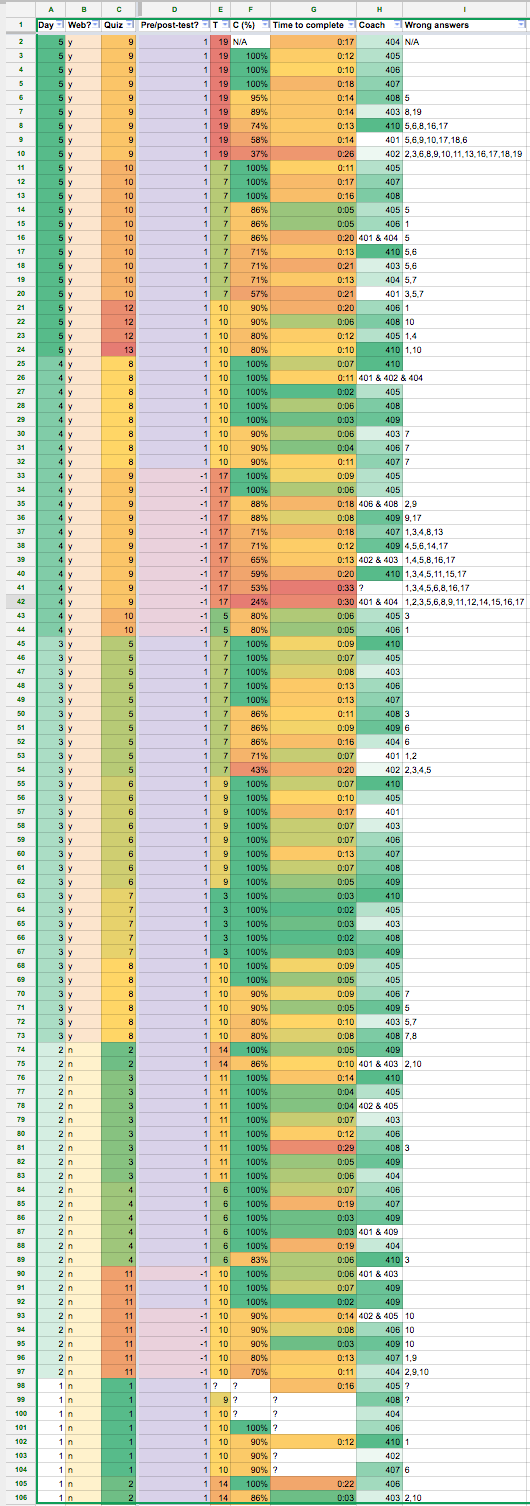
\includegraphics[width=0.5\textwidth]{analysis/sheets/zambiaResults.png}
        \caption{All quiz results from the Zambia coaches}
        \label{fig:zambiaResults}
    \end{figure}

    \clearpage

    There are some amount of coaches that have taken the same quizzes multiple times. From this, interesting conclusions can be drawn. Having taken the lecture before taking the quiz shows a 15.0\% average increase in quiz results, compared to an 12.8\% increase with simply taking the quiz two times. This shows that a lecture is still more effective than learning via the app.

    Time to finish a quiz took between 2 minutes to 33 minutes (3/4 quizzes that took longer than 25 minutes were on quiz 9, there is a correlation with number of questions). Most of the quizzes took under 5 minutes to complete, and results are always over 80\% for these instances. This shows that the coach had a high confidence with the answers. Similarly, all of the scores under 60\% has taken more than 20 minutes. This can be explained by that the coach is unfamiliar with the app or smartphone, and that the coach is uncertain of the answers.

    It is seen in the quiz results that the quizzes did get gradually more challenging, as the average of quiz scores gets lower after day 3 of training, when it was discovered was welcoming the quizzes to get harder.

    The quiz scores when quizzes are performed in group is very varying (from 24\% to 100\%), and it is observed that influence of another coach can lead both to a worse score than their individual average, and a higher score. It is interesting to see that the three coaches that have the worst average (67, 72 and 85\%) are also the ones that have taken quizzes the least times individually, and the most taking quizzes together with others. This may show that the app is more effective when used individually, and there seem no other connection to previous entrepreneurial activity or background.

    There are few correlations that can be made between the coach's background and experience, compared with quiz results or app behaviour, see again figure \ref{fig:zambiaSummary}. Nothing in the coach information distinguishes the worst 3 performers in the quiz. For the opposite, there is however a noticeable behaviour that being confident, having trained youth, leadership experience, business experience, care for community, care for oneself and confidence to take on many youth, almost guarantees a high quiz average (which demonstrates learning) and quizzes done (which demonstrates motivation).

    \begin{figure}[h]
        \centering
        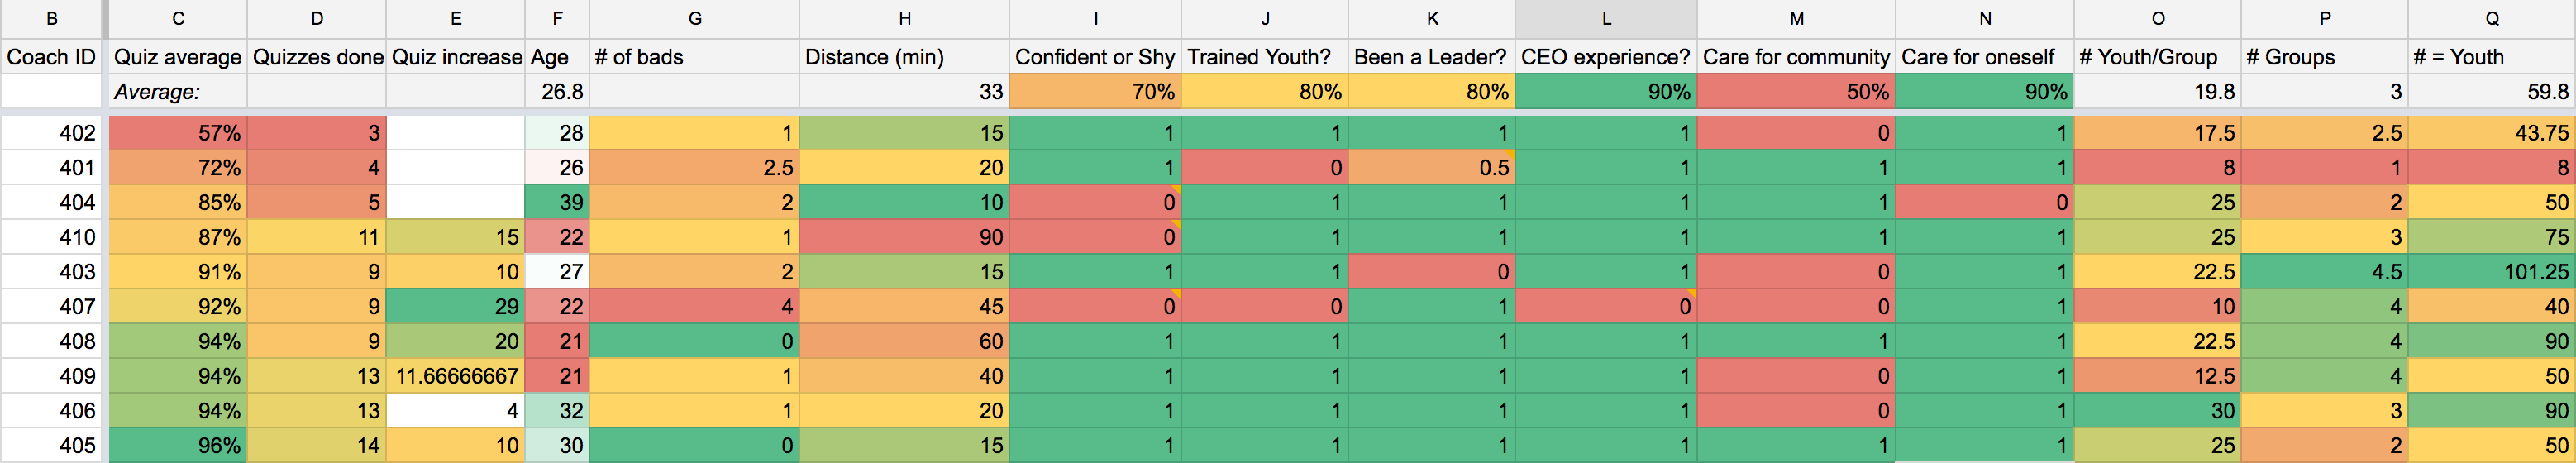
\includegraphics[width=1.0\textwidth]{analysis/sheets/zambiaSummary.png}
        \caption{Quiz results summary compared with data about a coach}
        \label{fig:zambiaSummary}
    \end{figure}

    For coaches with 0-1 negative remarks during the interviews (n=6) compared to coaches with 2-4 negative remarks (n=4), their quiz average is but 2\% higher (87\% to 85\%). This is not significant, but this number is increased to 93\% (an 8\% increase) if the outlier from the group is removed (a coach which only did three quizzes with average of 57\%). In the future, more research could be done into comparing coach data with quiz results.

    %Comparing instances when coaches have taken a test before and after a lecture, the results are: 71\%to 100\%, 59\% to 74\%, 80\% to 86\%, 90\% to 100\%. Without the lecture, improvements has been from 80 to 90, 100 to 100 to 100, 90 to 90, 80 to 100, 90 to 100, 100 to 100, 86 to 100, 100 to 100, 90 to 100.

    \subsubsection{Lessons Learned from App Test Observations}

    Below, lessons learned from the app tests are explained in regards to two categories: first by motivation aspects, and then by learning aspects.

    \subsubsubsection{Motivation}
    Regarding motivation from the coaches, one coach wished the app to be available on the Google Play store immediately, so that "The app could be used on my spare time". Another coach, without a smartphone, said "I'll buy one", because the utility of the app seemed so high. There were also suggestions for improvements, like "The app should have notes, not only quesitions". Regarding usability, low resolution screens made the text be barely visible. This showed, that the app needed to be tested on a lot of different devices. This is particularly true, as on day 1, the coaches did not know how to zoom, which could cause accident refreshs, frustration or confusion. Even more importantly, the app needs to work offline! To be online on the phone is too expensive for the coaches, and too unreliable to give a satisfactory experience. Also, during testing, relying on internet can cause a lot of problems, especially if the teacher is alone.

    When asked about what they thought about doing one quiz ("Graduation") as a pre-quiz (before the session), 10/10 said they liked doing the quiz before, and that it benefited their learning during the session. When asked why it helped, 10/10 said agreed on the statement "During session, it is easier to follow" and that "Giving the paper manuals before, scanning headings and pictures etc, would not help". So, using the quiz before the session increases learning, slightly decreases fun of the session, according to coaches. One of the coaches described it as "Fun and encouraging".

    It was also tested to work in group or individually. The ones who answered, said that you learned more individually (3/3), and more fun doing it together (3/3). Doing it together, was enjoyable as it was "Very easy because of using different minds" and "We can collaborate to do better". It can be argued that the quiz being easier is not a valid motivation, but describes the learning in the app as a desirable difficulty.

    When doing a post-quiz ("Goal setting") immediately afterwards versus at the end of the day (doing spaced versus massed learning), quotes were "I thought it was fun and challenging to do the quiz immediately afterwards", with another coach commenting "The mind was still fresh". After a discussion with the teacher, these were the results:

    %When asked on timing preference, 10/10 said it would be more fun to do the quiz immediately afterwards, not at the end of the day. The motivation, seemed to be that it was easier.

    %9/10, said they wanted to do the quiz afterwards. The outlier, said it would be better for learning doing it later.

    %After this comment, this was the distribution:

    \begin{itemize}
    \item 3/10 wants to do the quiz both before and after a session
    \item 1/10 wants to do the quiz before and at the end of the day
    \item 7/10 wants to do the quiz only immediately afterwards
    \item 10/10 wants to do the quiz immediately afterwards, and then again at the end of the day
    \item 7/10 wants to do the quiz immediately afterwards, and then a joined quiz with other topics at the end of the day
    \end{itemize}

    The high scores on using the app a lot indicates that they like the app. The teacher wants to listen to coach opinions, at the same time not spending more time than necessary on assessment.

    Regarding motivation from the teacher, discussion with Josefina what would hinder her from using the app, she says: "Not doing data collection digitally works whenever they are 10 - but not with bigger numbers than that." Also, she does not wish the app to replace her. She enjoys teaching, thinks she has an important role, and suggests the app to be designed to support her and the coaches, not replace her. When asked about what technical difficulties appeared with the app, she acknowledges that bugs in the app was sometimes a hindrance to use the app effortlessly, and that a lot of testing (both high-dose, and high-scale) is very important to acknowledge these.

    \subsubsubsection{Learning}
    Regarding assessing knowledge, coaches had surprisingly high quiz results, see figure \ref{zambiaSummary}, and at day 3 they wished harder questions when asked. The response was to give harder questions at the other days, for example by introducing similar answers, and testing 4 alternatives instead of 3. The changes were appreciated. The app was later tested on a university student in Uganda after the Zambia training, both on early and later quizzes. The university student from Makarere University scored 100\% correct, in spite of not having any entrepreneurship training. This showed that guessing was possible, or that the quizzes were too easy, a finding also shown by other tests with similar test subjects.

    The teacher Josefina commented that this might not be a problem, as the YoungDrive coaches are not as skilled with using a process of elimination, and had indeed scored lower results on average with the later quizzes. When testing the app with refugee innovators during Humanitarian Innovation Jam in Uganda, similar results to the YoungDrive coaches were found. She explains this because people in rural areas are not being equally educated and skilled with reasoning as university students, the problem is not as big as could be. Josefina is very happy with the app, and reviewed the app in the following way to Plan International after the training:

\textit{"The (YoungDrive coach training) app is a great tool to measure how much the coaches learned and understood from the daily training; it provides a clear overview of what the coaches truly understood and what they actually still don’t completely understand. Based on that information I as a tutor can adjust the training for the following day to make sure that the coaches understand everything correctly. The app also works as a motivator for the coaches; it´s clearly reflect their own daily performances. If they score high they become very happy and satisfied, if they score low they are eager to check their wrong answers.".}

A coach scoring only 9/19 showed the relevancy of the quiz, as Josefina did not think she would have discovered that the coach was lagging behind otherwise. In the data, it was observable that the coach had done well together with others, but 3/7 when done individually. Josefina said about the 9/19: "This is where a control group would be beneficial". "He is often passive during open questions, but active during the team exercises."

According to Josefina, if you have a high score, you are ready. If not, you need to redo the quiz. If you are 8/10 or lower, you are in the red zone. If lower than 10/10, they are not ready, the motivation being that what they don't know, they will teach in an improper way: affecting hundreds of youth. This is why Josefina thinks they should need all of the answers correct. Getting all of the answers correct can be supported by the literature, especially on deliberate practice where 95\% reliability in the topic is needed for maximum effectiveness \citep{sierra}.

Up until now, merely Correct Information has been assessed, not the other three factors. The fact that the app already is appreciated with assessing Correct Information, makes starting to assess the other factors interesting. Josefina informs that Correct Structure, Time Management and Fun Atmosphere would be the most viable to test \textit{after} a youth session, not before. She notes, that \textit{some} assessment could be made via the app before a session. This could to be further investigated.
